% !TeX TXS-program:compile = txs:///lualatex

\documentclass[a4paper,11pt]{article}
\usepackage[breakable]{cp-base}
\graphicspath{{./graphics/}}
%variables
\donnees[%
	typedoc=CHAPITRE~,
	numdoc=7,
	classe=1\up{ère} 2M2,
	matiere={[SPÉ.MATHS]},
	annee=2021,
	titre={Nombre dérivé, tangente}
	]

%formatage
\author{Pierquet}
\title{\nomfichier}
\hypersetup{pdfauthor={Pierquet},pdftitle={\nomfichier},allbordercolors=white,pdfborder=0 0 0,pdfstartview=FitH}
%divers
\lhead{\entete{\matiere}}
\chead{\entete{\lycee}}
\rhead{\entete{\classe{} - Chapitre \thepart}}
\lfoot{\pied{\matiere}}
\cfoot{\logolycee{}}
\rfoot{\pied{\numeropagetot}}

\begin{document}

\pagestyle{fancy}

\part{CH07 - Dérivation locale}

\section{Taux d'accroissement}

\begin{ccadre}
Soit $I$ un intervalle contenant les deux nombres distincts $a$ et $b$.

Soit $f$ une fonction définie sur $I$, et $\mathscr{C}_f$ sa courbe représentative.
\end{ccadre}

\begin{cdefi}
On appelle \textbf{taux d'accroissement de $f$ entre $a$ et $b$} le quotient noté $t_{f,a,b}$ égal à : \[\frac{f(b)-f(a)}{b-a}.\]%
Graphiquement, le taux d'accroissement de $f$ entre $a$ et $b$ est la \textbf{pente de la droite $(AB)$} où $A$ et $B$ sont les points de $\mathscr{C}_f$ d'abscisses respectives $a$ et $b$.
\end{cdefi}

\begin{cillustr}
\vspace{-0.2cm}
\begin{center}
	\tikzset{cross/.style={%
			cross out, draw=black, minimum size=2*(#1-\pgflinewidth), inner sep=0pt, outer sep=0pt},
			cross/.default={1pt}}
	\tunits{0.7}{0.7}
	\tdefgrille{-1}{8}{1}{1}{-1}{5}{1}{1}
	\begin{tikzpicture}[x=\xunit cm,y=\yunit cm]
		\tgrilles[line width=0.6pt,densely dotted,lightgray] ;
		\axestikz* ;
		\draw[line width=1.5pt,->,>=stealth] (0,0) -- (0,1) ;
		\draw[line width=1.5pt,->,>=stealth] (0,0) -- (1,0) ;
		\clip (-2,\ymin) rectangle (\xmax,\ymax) ;
		\draw[line width=1.pt,ForestGreen,domain=\xmin:\xmax,samples=450] plot (\x,{0.5*\x*\x-4*\x+7.5});
		\draw[darkgray,line width=1pt,densely dashed] (2,0) -- (2,1.5) -- (0,1.5) ;
		\draw[darkgray,line width=1pt,densely dashed] (7,0) -- (7,4) -- (0,4) ;
		\draw[line width=1.pt,purple,domain=\xmin:\xmax,samples=450] plot (\x,{0.5*\x+0.5});
		\foreach \Point/\Val/\Pos in {(2,0)/a/below,(7,0)/b/below,(0,1.5)/f(a)/left,(0,4)/f(b)/left}
		{\draw \Point node[\Pos] {\footnotesize $\Val$} ;
			\draw[thick] \Point node[cross=2.5pt]{};}
		\foreach \Point/\Val/\Pos in {(2,1.5)/$A$/above right,(7,4)/$B$/above left}
		{\draw \Point node[blue,\Pos] {\small \Val} ;
			\draw[blue,fill=blue!50] \Point circle[radius=2pt] ;}
	\end{tikzpicture}
\end{center}
\end{cillustr}

\begin{crmq}
La courbe ayant pour équation $y=f(x)$, on a donc $t_{f,a,b}=\frac{\Delta y}{\Delta x}$.

\smallskip

Si, en physique par exemple, la fonction mesure l'évolution d'une quantité $C$ en fonction du temps $t$, le taux d'accroissement se notera plutôt $\frac{\Delta C}{\Delta t}$.
\end{crmq}

\begin{cexemple}
Si on considère la fonction définie par $f(x)=0,5x^2-4x+7,5$ représentée ci-dessus, le taux d'accroissement de $f$ entre 2 et 7 est : \vspace{-0.1cm} \[t_{f,2,7}=\frac{f(7)-f(2)}{7-2}=\frac{4-1,5}{7-2}=\frac{1}{2}.\]
\end{cexemple}

\section{Nombre dérivé}

\begin{cintro}
Considérons un point $A$ fixe sur la courbe $\mathscr{C}_f$, d'abscisse $a$, et un point $M$ \textbf{mobile} sur la même courbe, d'abscisse $a+h$ ($h$ correspondant donc à l'\emph{écart} entre $A$ et $M$ sur l'axe des abscisses).

Le taux d'accroissement de $f$ entre $a$ et $a+h$ se note donc \[t_{f,a,a+h}=\frac{f(a+h)-f(a)}{h}.\]
\end{cintro}

\begin{cdefi}
Si le taux d’accroissement de $f$ entre $a$ et $a+h$ devient aussi proche que l’on veut d’une valeur limite $l\in\R$ lorsque $h$ se rapproche de 0, on dit que la fonction $f$ est \textbf{dérivable en $a$}.

La valeur limite $\ell$ est alors appelée \textbf{nombre dérivé de $f$ en $a$}, que l’on note $f'(a)$. On a alors : \[\lim\limits_{h \rightarrow 0} \frac{f(a+h)-f(a)}{h}=f'(a).\]
\end{cdefi}

\begin{clog}
Avec la même fonction que ci-dessus, $f(x)=0,5x^2-4x+7,5$ et $a=2$, on \csheet{tabule} le taux d'accroissement :
\begin{center}
	\includegraphics[width=12cm]{chap07_tab_derive}
\end{center}
On remarque bien que le taux d'accroissement \textbf{semble} se rapprocher de $\textcolor{ForestGreen}{-2}$ lorsque $h$ tend vers 0.

On peut démontrer ce résultat par le calcul :

$\bullet~~$le taux d'accroissement de $f$ entre $\textcolor{orange}{2}$ et $\textcolor{orange}{2}+h$ est $\frac{\textcolor{blue}{ f(\textcolor{orange}{2}+h)}-\textcolor{red}{f(\textcolor{orange}{2})}}{h}$ ;

$\bullet~~$\color{red} $f(\textcolor{orange}{2})=0,5 \times \textcolor{orange}{2}^2-4 \times \textcolor{orange}{2} +7,5=1,5$

\color{black}$\bullet~~$\color{blue}$f(\textcolor{orange}{2}+h)=0,5(\textcolor{orange}{2}+h)^2-4(\textcolor{orange}{2}+h)+7,5=0,5(4+4h+h^2)-8-4h+7,5=2+2h+0,5h^2-8-4h+7,5=0,5h^2-2h+1,5$

\color{black}$\bullet~~$donc le taux d'accroissement est $\frac{\textcolor{blue}{0,5h^2-2h+1,5}-\textcolor{red}{1,5}}{h}=\frac{0,5h^2-2h}{h}=\frac{h(0,5h-2)}{h}=0,5h-2$.

\smallskip

Ainsi, lorsque $h$ tend vers 0, le taux d'accroissement tend vers $0,5 \times 0 -2=-2$

Le nombre dérivé de $f$ en 2 est $f'(2)=\textcolor{ForestGreen}{-2}$ !
\end{clog}	

\begin{crmq}
Il est possible que le taux d'accroissement ne se rapproche pas d'une valeur particulière, ou qu'il se rapproche de l'infini quand $h$ tend vers 0. Dans ce cas, la fonction n'est pas dérivable. C'est le cas par exemple de la fonction racine carrée avec $a=0$ :

En effet, le taux d'accroissement de la fonction racine carrée entre 0 et $0+h$ est : \[\frac{\sqrt{0+h}-\sqrt{0}}{h}=\frac{\sqrt{h}}{h}=\frac{\sqrt{h}}{\sqrt{h} \times \sqrt{h}}=\frac{1}{\sqrt{h}}\] qui se rapproche de l'infini lorsque $h$ tend vers 0 !
\end{crmq}

\begin{cillustr}
\uline{Graphiquement}, que se passe-t-il ?
\renewcommand{\arraystretch}{2}
{\small \begin{center}
	\begin{tabularx}{\linewidth}{|Y|Y|Y|Y|}
	\cline{2-4}
	\multicolumn{1}{c|}{}& \textbf{Le point M} & \textbf{La droite (AM)} & \textbf{Le taux d'accroissement} \\
	\hline
	\textbf{Lorsque $\grasmaths{h}$ varie} & se déplace sur la courbe & pivote autour de $A$ & varie \\
	\hline
	\textbf{Lorsque $\grasmaths{h=0}$} & se confond avec $A$ & disparaît & n'existe pas \\
	\hline 
	\textbf{Lorsque $\grasmaths{h}$ tend vers 0 }& se rapproche de $A$ & "frôle" la courbe & se rapproche d'un nombre \\
	\hline 
\end{tabularx} 
\end{center}}
\end{cillustr}

\section{Tangente}

\begin{cdefi}
Si la courbe $\mathscr{C}_f$ d'une fonction $f$ est bien \og lisse \fg{} au voisinage d'un point $A$, on appelle \textbf{tangente} à $\mathscr{C}_f$ en $A$ une droite qui épouse localement la direction de cette courbe. Autrement dit, en zoomant autour du point $A$, la courbe va finir par sembler se confondre avec sa tangente en ce point.

\begin{center}
	\tunits{0.5}{0.5}
	\tdefgrille{-1}{9}{2}{2}{-2}{8}{2}{2}
	\begin{tikzpicture}[x=\xunit cm,y=\yunit cm]
		\filldraw[white] (\xmin,\ymin) rectangle (\xmax,\ymax) ;
		\tgrilles[line width=0.4pt,lightgray] ;
		\axestikz*[width=1pt] ;
		\clip (\xmin,\ymin) rectangle (\xmax,\ymax) ;
		\draw[line width=1pt,ForestGreen,domain=\xmin:\xmax,samples=250] plot (\x,{0.5*(\x-4)*(\x-4)-0.5}) ;
		\draw[line width=1pt,NavyBlue,domain=\xmin:\xmax] plot (\x,{1.8*(\x-5.8)+1.12}) ;
		\draw[line width=1pt,red,fill=red!50,opacity=0.5] (5.8,1.12) circle[radius=2] ;
		\filldraw[darkgray] (5.8,1.12) circle[radius=2.5pt] ; 
	\end{tikzpicture}
	~~
	\tunits{2}{2}
	\tdefgrille{-1}{9}{2}{0.5}{-2}{8}{2}{0.5}
	\begin{tikzpicture}[x=\xunit cm,y=\yunit cm]
		\clip (4.55,-0.13) rectangle (7.05,2.37) ;
		\filldraw[white] (\xmin,\ymin) rectangle (\xmax,\ymax) ;
		\tgrilles[line width=0.4pt,lightgray] ;
		\axestikz*[width=1pt] ;
		\draw[line width=1pt,ForestGreen,domain=\xmin:\xmax,samples=250] plot (\x,{0.5*(\x-4)*(\x-4)-0.5}) ;
		\draw[line width=1pt,NavyBlue,domain=\xmin:\xmax] plot (\x,{1.8*(\x-5.8)+1.12}) ;
		\draw[line width=1pt,red,fill=red!50,opacity=0.5] (5.8,1.12) circle[radius=1] ;
		\filldraw[darkgray] (5.8,1.12) circle[radius=2.5pt] ; 
	\end{tikzpicture}
	~~
	\tunits{10}{10}
	\tdefgrille{-1}{9}{2}{0.1}{-2}{8}{2}{0.1}
	\begin{tikzpicture}[x=\xunit cm,y=\yunit cm]
		\clip (5.55,0.87) rectangle (6.05,1.37) ;
		\filldraw[white] (\xmin,\ymin) rectangle (\xmax,\ymax) ;
		\tgrilles[line width=0.4pt,lightgray] ;
		\axestikz*[width=1pt] ;
		\draw[line width=1pt,ForestGreen,domain=\xmin:\xmax,samples=250] plot (\x,{0.5*(\x-4)*(\x-4)-0.5}) ;
		\draw[line width=1pt,NavyBlue,domain=\xmin:\xmax] plot (\x,{1.8*(\x-5.8)+1.12}) ;
		\draw[line width=1pt,red,fill=red!50,opacity=0.5] (5.8,1.12) circle[radius=1] ;
		\filldraw[darkgray] (5.8,1.12) circle[radius=2.5pt] ; 
	\end{tikzpicture}
\end{center}
\end{cdefi}

\begin{crmq}
Avec les notations précédentes, lorsque $h$ tend vers 0, la position \textbf{limite} de la droite $(AM)$ est la \textbf{tangente} $\mathscr{T}_a$ à la courbe $\mathscr{C}_f$ en $a$.

Donc la valeur limite de la pente de $(AM)$ est la pente de la tangente.

Ainsi, le nombre dérivé $f'(a)$ est la \textbf{pente de la tangente} au point d'abscisse $a$.
\end{crmq}

\begin{cprop}[ : interprétation graphique du nombre dérivé]
Le \textbf{nombre dérivé} $f'(a)$ est la \textbf{pente de la tangente} à $\mathscr{C}_f$ au point d'abscisse $a$.

Cette tangente, au point d'abscisse $a$, a donc pour équation : \[y=f'(a) \times (x-a)+f(a).\] 
\end{cprop}

\begin{cdemoblanc}
La tangente au point d'abscisse $a$ est une droite d'équation $y=mx+p$.

On sait que sa pente est $p=f'(a)$, et on sait qu'elle passe par le point $A(a\,;\,f(a))$ donc les coordonnées de $A$ doivent vérifier $y_A=f'(a) \times x_A+p$ soit $f(a)=f'(a) \times a+p$ donc $p=f(a)-f'(a) \times a$.

L'équation de la tangente est donc $y=f'(a)\times x+f(a)-f'(a) \times a=f'(a) \times (x-a)+f(a)$.
\end{cdemoblanc}

\begin{cexemple}
Toujours avec le même exemple, on a prouvé par le calcul que le nombre dérivé était $f'(\textcolor{orange}{2})=\textcolor{ForestGreen}{-2}$.

On peut vérifier graphiquement que la tangente au point d'abscisse \textcolor{orange}{$2$} a bien une pente égale à \textcolor{ForestGreen}{$-2$}. 

\begin{center}
	\tunits{1.5}{1.5}
	\tdefgrille{-1}{7}{1}{1}{-1}{4}{1}{1}
	\begin{tikzpicture}[x=\xunit cm,y=\yunit cm]
		\draw[line width=1.25pt,red,fill=red!15] (2,1.5) -- (3,1.5) -- (3,-0.5) -- cycle ; 
		\tgrilles[line width=0.6pt,densely dotted,lightgray] ;
		\axestikz* ;
		\draw[line width=1.5pt,->,>=stealth] (0,0) -- (0,1) ;
		\draw[line width=1.5pt,->,>=stealth] (0,0) -- (1,0) ;
		\draw[line width=1.25pt,red] (2,1.5) -- (3,1.5) -- (3,-0.5) ;
		\clip (\xmin,\ymin) rectangle (\xmax,\ymax) ;
		\draw[darkgray,line width=1pt,densely dashed] (2,0) -- (2,1.5) -- (0,1.5) ;
		\draw[line width=1.5pt,ForestGreen,domain=\xmin:\xmax,samples=450] plot (\x,{0.5*\x*\x-4*\x+7.5});
		\draw[line width=1.5pt,purple,domain=\xmin:\xmax,samples=450] plot (\x,{-2*\x+5.5});
		\draw[blue,fill=blue!50] (2,1.5) circle[radius=2pt] node[above right] {\blue $A$} ;
		\draw[red] (2.75,1.66) node {$+1$} (3.25,0.5) node {$-2$} ;
		\draw[red] (1.5,2.5) node[left] {$y=-2x+5,5$} ;
	\end{tikzpicture}
\end{center}
La tangente a donc pour équation $y=\textcolor{ForestGreen}{f'(2)}\times (x-\textcolor{gray}{2})+\textcolor{red}{f(2)}$ soit  $y=\textcolor{ForestGreen}{-2}\times (x-\textcolor{gray}{2})+\textcolor{red}{1,5}$ ou encore, en développant, $y=-2x+5,5$.
\end{cexemple}

\begin{cloglogo}{windows}
\begin{center}
	\begin{tikzpicture}[x=1cm,y=1cm,line width=1pt]
		\paramCF[larg=15,esplg=3pt,color=darkgray,menu=true,size=\normalsize,%
		poscmd=left,titre=true,labeltitre=Logiciel de Calcul Formel Xcas]
		\ligneCF[hc=0.75,hr=0.75]{$\mathsf{f(x):=0.5*x\chap2-4*x+7.5}$}{$\mathsf{x \mapsto 0.5*x^2-4*x+7.5}$}
		\ligneCF[hc=0.75,hr=0.75]{$\mathsf{m:=limite(taux\_accroissement(f(x),2,2+h),h,0)}$}{$\mathsf{-2}$}
		\ligneCF[hc=0.75,hr=0.75]{$\mathsf{developper(m*(x-2)+f(2))}$}{$\mathsf{-2*x+5.5}$}
		\ligneCF[hc=0.75,hr=0.75]{$\mathsf{equation(tangente(plotfunc(f(x)),2))}$}{$\mathsf{-2*x+5.5}$}
	\end{tikzpicture}
\end{center}
\end{cloglogo}

\end{document}